\documentclass[12pt]{article}
\usepackage[utf8]{inputenc}
\usepackage[english]{babel}
\usepackage{amsmath}
\usepackage{natbib}
\usepackage{adjustbox}
\usepackage{listings}
\usepackage{graphicx}
\usepackage{hyperref}
\usepackage[english]{babel}
\usepackage[T1]{fontenc}
\usepackage[utf8]{inputenc}
\usepackage{caption}
\usepackage{caption,float}
\usepackage[vmargin=3cm,hmargin=3cm]{geometry}

\begin{document}

{\centering

\rule{\textwidth}{1.6pt}\vspace*{-\baselineskip}\vspace*{2pt} 
\rule{\textwidth}{0.4pt}\\[\baselineskip] 
{\LARGE Analyzing the Weekly S\&P Stock Market Data using Logistic Regression}
\rule{\textwidth}{0.4pt}\vspace*{-\baselineskip}\vspace{3.2pt}
\rule{\textwidth}{1.6pt}\\[\baselineskip] 

\vspace{20mm} %5mm vertical space
\scshape % Small caps
CMSC 6950 - Computer Based Research Tools and Applications \\ [\baselineskip]
Term Project \\[\baselineskip] 
6th August, 2020 \\[\baselineskip] 
\vspace{20mm} %5mm vertical space
Submitted by \\[\baselineskip]
{\Large Kwadwo Nyame Owusu-Boakye \\ (201990860) \par}
\vfill
{\itshape Memorial University of Newfoundland \\ St. John's, Canada.\par} 
}

\newpage

{\centering
  \section*{Abstract}
}
The main focus of the project is to analyze the Weekly S\&P Stock Market Data using logistic regression. The Logistic Regression was first used to model the Weekly S\&P Stock Market Data. It was observed that the intercept and Lag 2 were the only significant ones. The logistic regression was again used to model Lag 2 and also used to model the interaction between Lag1 and Lag2. It was seen that the logistic model with one predictor (Lag 2) gave the  best results because of the maximum model accuracy (overall fraction of correct prediction).

\section{Introduction}
The S\&P 500, or basically the S\&P, is a stock exchange index that evaluates the stock performance of 500 huge companies recorded on stock trades in the United States. It is one of the most usually followed equity indicators, and many believe it to be probably the best depictions of the U.S. stock exchange. The normal yearly aggregate return of the index, including profits, since beginning in 1926 has been 9.8\%; be that as it may, there were more than a few years where the index dropped over 30\%. The index has posted yearly increases 70\% of the time (\cite{ref-wiki}) .\\\\
The index is one of the components in calculation of the Conference Board Leading Economic Index, used to predict the course of the economy. The index is related with numerous ticker images, including: \^GSPC, INX, and \$SPX, dependent on marketplace or internet site. The index value is revised each 15 seconds, or 1,559 times per business day, with price upgrade circulated by Reuters (\cite{ref-quote}).


\section{Materials and Methods}
\subsection{Logistic Regression}
Let attempt to comprehend logistic regression by thinking about a logistic model with given parameters, at that point perceiving how the coefficients can be assessed from data. Think about a model with two forecasters, {${\displaystyle x_{1}}$} and {${\displaystyle x_{2}}$}, and single binary (Bernoulli) response variable {${\displaystyle Y}$}, which we represent {${\displaystyle p=P(Y=1)}$}. We believe a linear correlation sandwiched between the predictor variables and the log-odds of the outcome that {${\displaystyle Y=1}$}. This linear correlation* can be written in the ensuing mathematical structure (where {${\displaystyle \ell}$} is the log-{}odds, {${\displaystyle b}$} is the base of the logarithm, and {${\displaystyle \beta _{i}}$} are parameters of the model):
\begin{equation}
	{{\displaystyle \ell =\log _{b}{\frac {p}{1-p}}=\beta _{0}+\beta _{1}x_{1}+\beta _{2}x_{2}}}
\end{equation}
We can retrieve the log-odds:
\begin{equation}
	{{\displaystyle {\frac {p}{1-p}}=b^{\beta _{0}+\beta _{1}x_{1}+\beta _{2}x_{2}}}}.
\end{equation}
By straightforward algebraic manipulation, the likelihood that {${\displaystyle Y=1}$} is
\begin{equation}
	{{\displaystyle p={\frac {b^{\beta _{0}+\beta _{1}x_{1}+\beta _{2}x_{2}}}{b^{\beta _{0}+\beta _{1}x_{1}+\beta _{2}x_{2}}+1}}={\frac {1}{1+b^{-(\beta _{0}+\beta _{1}x_{1}+\beta _{2}x_{2})}}}}}.
\end{equation}
The equation above reveals that as soon as {${\displaystyle \beta _{i}}$} are fixed, we can effortlessly calculate either the log-odds that {${\displaystyle Y=1}$} for a given observation, or the likelihood that {${\displaystyle Y=1}$} for a given observation. The main usage of a logistic model is to be provided an observation {${\displaystyle (x_{1},x_{2})}$}, and calculate the likelihood {${\displaystyle p}$} that {${\displaystyle Y=1}$}. In many applications, the base {${\displaystyle b}$} of the logarithm is generally taken to be {${\displaystyle e}$}. Nevertheless, in some cases it can be simpler to convey results by working in base 2, or base 10 (\cite{ref-wiki:xxx}).

\subsection{Data Collection and Description}
In this project, the dataset used was downloaded or collected online from (\url{https://www.picostat.com/dataset/r-dataset-package-islr-weekly}) by executing a pandas python code. \\\\
This dataset consists of percentage returns for the stock index over 1089 weeks for 21 years, from the beginning of 1990 to the end of 2010.  For each data,  we have the percentage returns for each of the  first previous trading weeks, Lag1 through Lag5.  We have also Volume (the number of shares traded on the previous day, in billions), Today (the percentage return on the date in question) and Direction (whether the market was Up or Down on this date). 

\subsection{Python-Software Packages Used}
The dataset downloaded was then analyzed mainly using three open source python packages. These packages are Pingouin, Statsmodels and PyCM packages. \\\\
The Pingouin package was used to determine the structure, summary, correlation, normality of variables in the dataset and also analyze the dataset with the logistic regression model (\cite{ref-software}). The Statsmodel was then used to determine the Confusion matrix of the logistic regression output derived. Lastly, the PyCM package was used to check the performance or accuracy or predictions of these models (\cite{ref-softwaree}).


\section{Analysis and Results}
\subsection{Numerical and Graphical Summaries of Data}

\subsubsection{Structure of Data}
The Table~\ref{table_1} below shows the structure of the dataset used. This data consists of percentage returns for the stock index over 1089 weeks for 21 years, from the beginning of 1990 to the end of 2010. For each column, we have the percentage returns for each of the first previous trading weeks, Lag1 through Lag5. We have also Volume, Today and Direction. 


\begin{table}[h!]
\begin{tabular}{rrrrrrrrl}
	\hline
	Year &   Lag1 &   Lag2 &   Lag3 &   Lag4 &   Lag5 &    Volume &  Today & Direction \\
	\hline
	1990 &  0.816 &  1.572 & -3.936 & -0.229 & -3.484 &  0.154976 & -0.270 &      Down \\
	1990 & -0.270 &  0.816 &  1.572 & -3.936 & -0.229 &  0.148574 & -2.576 &      Down \\
	1990 & -2.576 & -0.270 &  0.816 &  1.572 & -3.936 &  0.159837 &  3.514 &        Up \\
	1990 &  3.514 & -2.576 & -0.270 &  0.816 &  1.572 &  0.161630 &  0.712 &        Up \\
	1990 &  0.712 &  3.514 & -2.576 & -0.270 &  0.816 &  0.153728 &  1.178 &        Up \\
	\hline
\end{tabular}
\caption{Structure of Data}
\label{table_1}
\end{table}

\subsubsection{Descriptive Statistics of Data}

From Table~\ref{table_2}, we can see the statistics of the variables employed for this study. This includes the count, minimum, maximum, mean, median (50\%), 1st quartile (25\%) and 3rd quartile (75\%).\\\\
It can be observed that Lag 5 has the highest standard deviation value of 2.361285 indicating that Lag 5 had the highest level of impact on Direction. Also, Volume had the least level of impact due to its low standard deviation value (1.686636)


\begin{table}[h!]

 \resizebox{\textwidth}{!}{ 
	\begin{tabular}{rrrrrrrrr}
		\hline
	&	Year &         Lag1 &         Lag2 &         Lag3 &         Lag4 &         Lag5 &       Volume &        Today \\
		\hline
	count&	1089.000000 &  1089.000000 &  1089.000000 &  1089.000000 &  1089.000000 &  1089.000000 &  1089.000000 &  1089.000000 \\
	mean	&2000.048669 &     0.150585 &     0.151079 &     0.147205 &     0.145818 &     0.139893 &     1.574618 &     0.149899 \\
		std&6.033182 &     2.357013 &     2.357254 &     2.360502 &     2.360279 &     2.361285 &     1.686636 &     2.356927 \\
		min&1990.000000 &   -18.195000 &   -18.195000 &   -18.195000 &   -18.195000 &   -18.195000 &     0.087465 &   -18.195000 \\
		25\%&1995.000000 &    -1.154000 &    -1.154000 &    -1.158000 &    -1.158000 &    -1.166000 &     0.332022 &    -1.154000 \\
		50\%&2000.000000 &     0.241000 &     0.241000 &     0.241000 &     0.238000 &     0.234000 &     1.002680 &     0.241000 \\
		75\%&2005.000000 &     1.405000 &     1.409000 &     1.409000 &     1.409000 &     1.405000 &     2.053727 &     1.405000 \\
		max&2010.000000 &    12.026000 &    12.026000 &    12.026000 &    12.026000 &    12.026000 &     9.328214 &    12.026000 \\
		\hline
	\end{tabular}
}
\caption{Descriptive Statistics of Data}
\label{table_2}
\end{table}

\subsubsection{Normality Test of Variables}

Here, the Pingouin python package was used to check for normality in the variables. The normal distribution fit of the independent variables  (Lag 1, Lag 2, Lag 3, Lag 4, Lag 5, Volume, Today) is seen in the Table~\ref{table_3}.\\\\
It can be seen from the table that none of the independent variables was normal. In other words, they all showed signs of skewness.

\begin{table}[h!]
	\centering
	
\begin{tabular}{rrrl}
\hline
&	W &          pval &  normal \\
\hline
Year&	0.950223 &  9.951609e-19 &   False \\
Lag 1&	0.948756 &  5.232496e-19 &   False \\
Lag 2&	0.948813 &  5.364750e-19 &   False \\
Lag 3&	0.949282 &  6.578534e-19 &   False \\
Lag 4&	0.949279 &  6.570206e-19 &   False \\
Lag 5&	0.949428 &  7.011749e-19 &   False \\
Volume&	0.787729 &  2.101803e-35 &   False \\
Today&	0.948765 &  5.252924e-19 &   False \\
\hline
\end{tabular}
\caption{Normality Test of Variables}
\label{table_3}
\end{table}

\subsection{Correlation Analysis}

\subsubsection{Graphical Summary of Data}

\begin{figure}[!htbp]
	\centering
	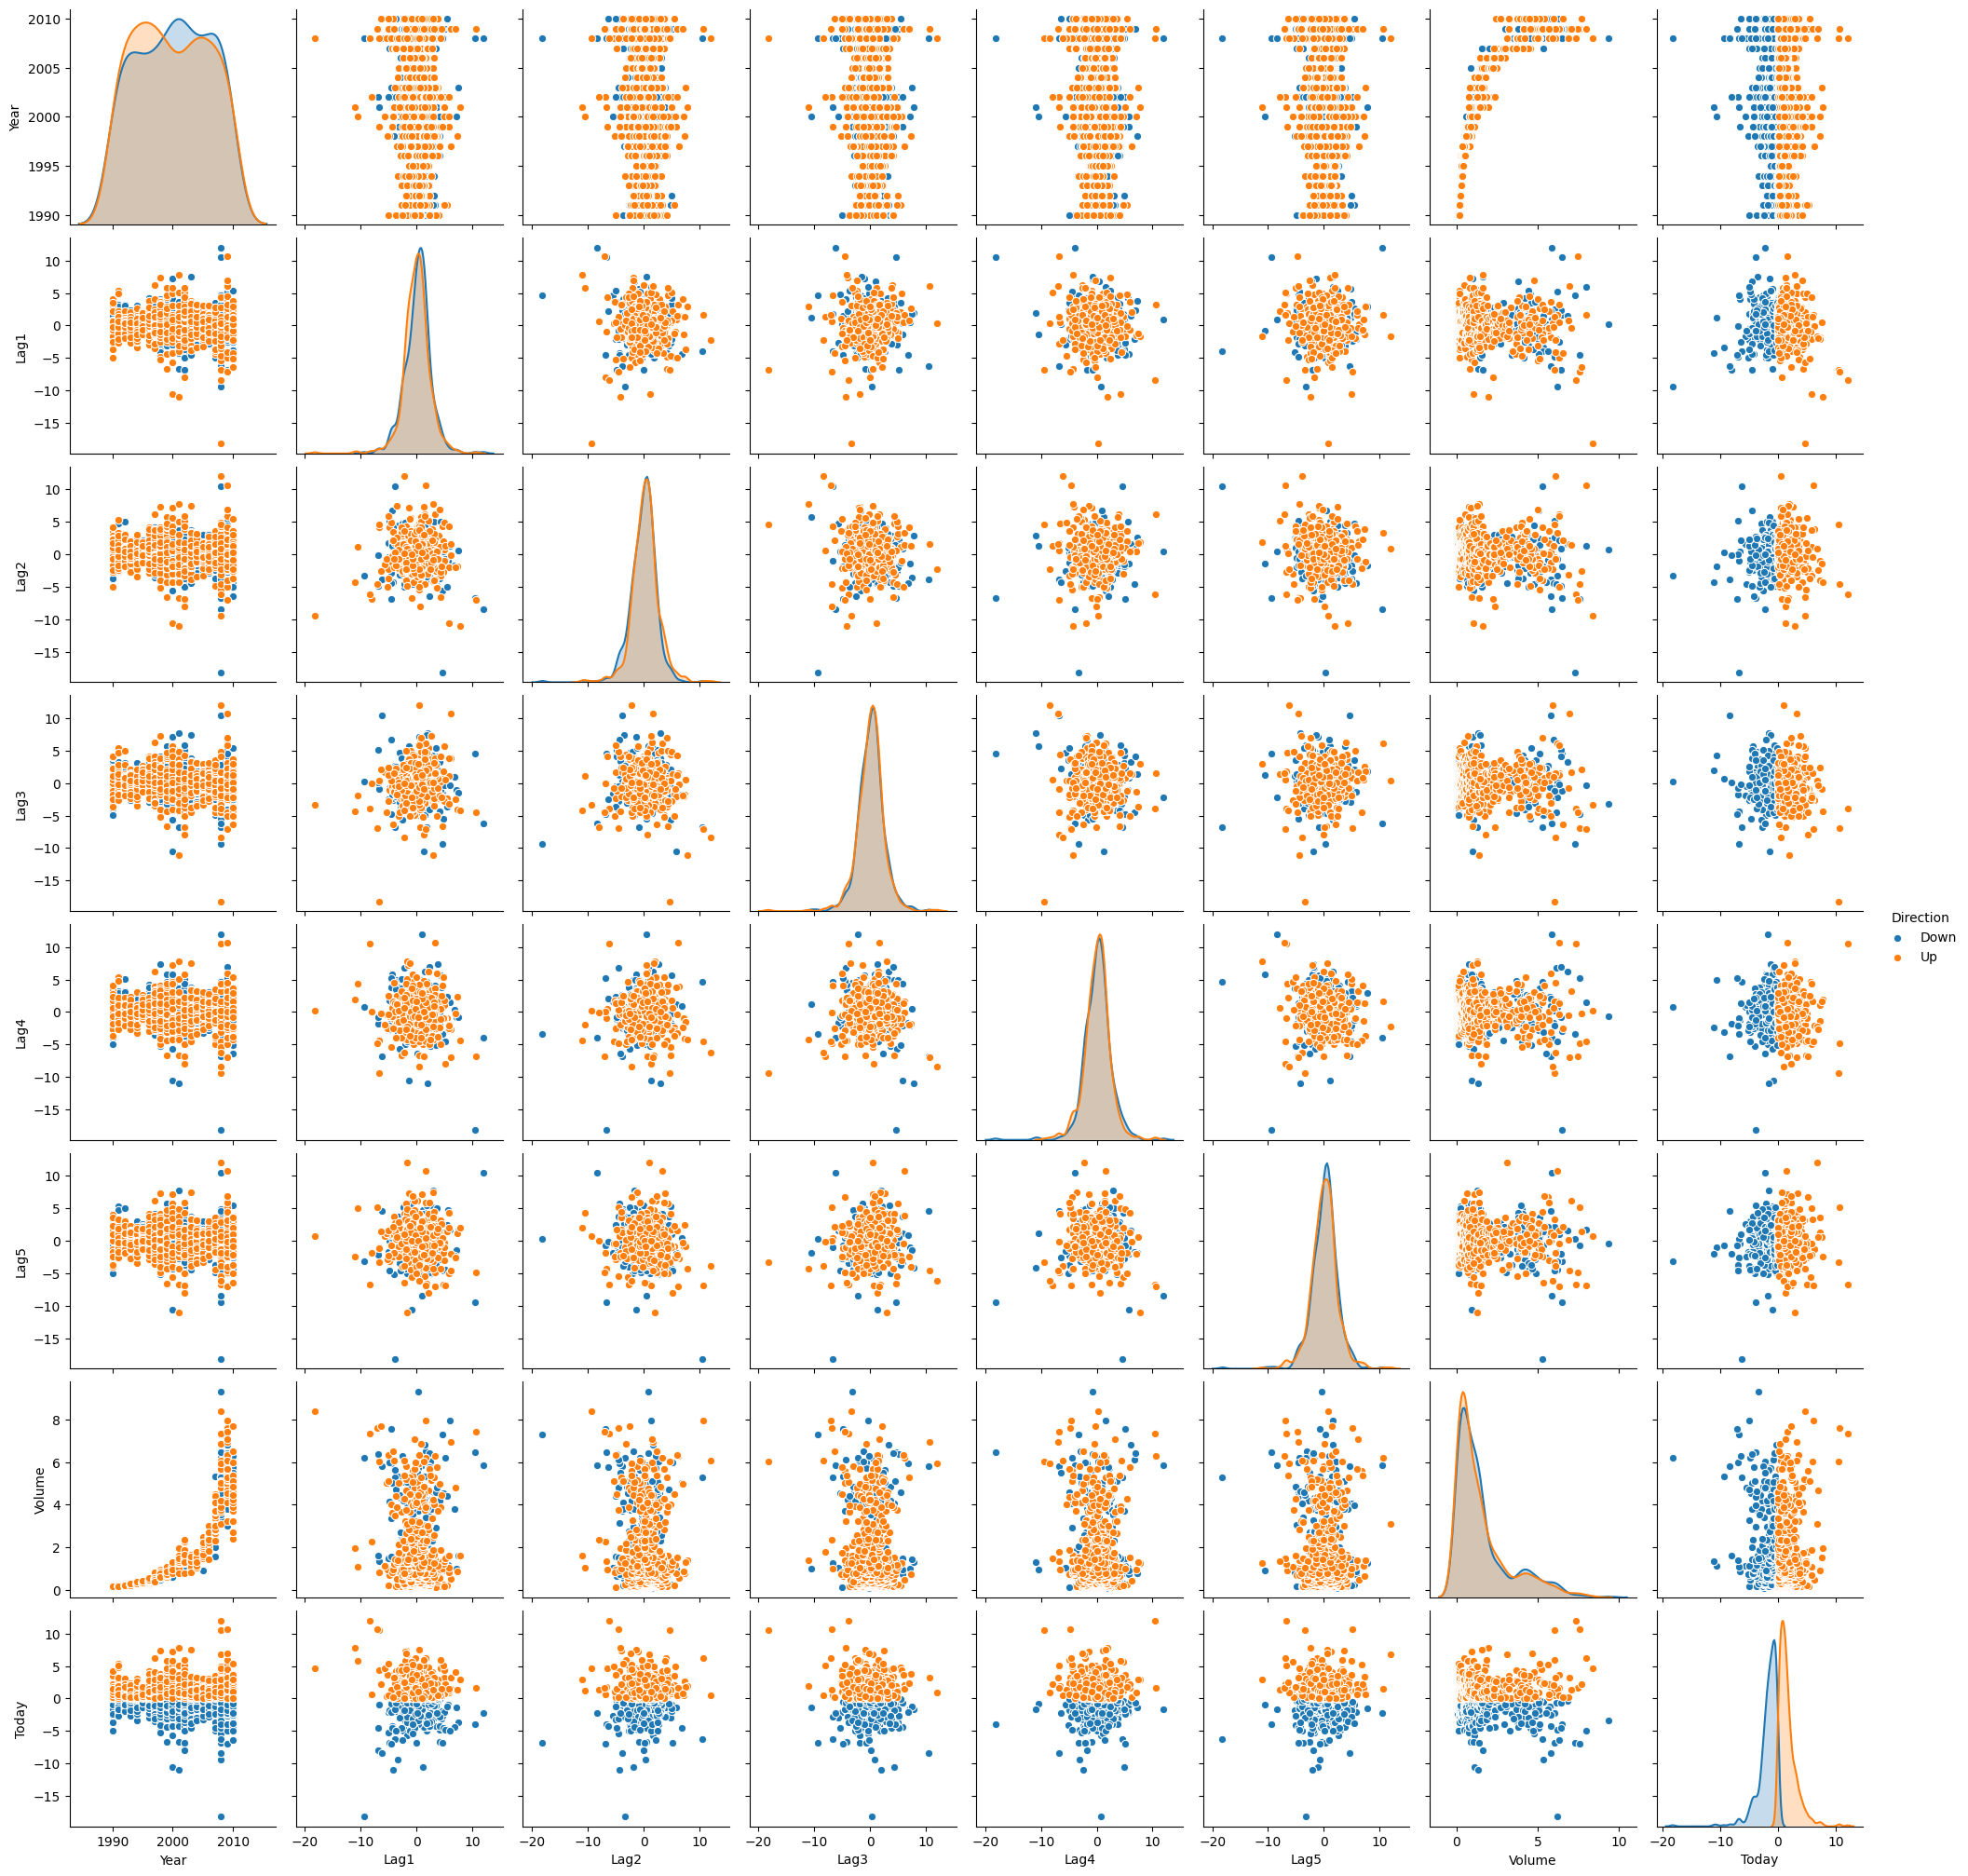
\includegraphics[width=12 cm]{graphical_summary_of_data.png}
	\caption{Graphical Summary of Correlation between Variables}
	\label{fig_1}
\end{figure}

From Table~\ref{table_1}, Table~\ref{table_2} and Figure~\ref{fig_1}, some years seem to have more or less variations than others. Looking at the shape of the various Lag features and the Year. There does seem to be some autocorrelation in the variability of the Lags and the year. Perhaps some years, people are more skittish than other years, and this takes a while to wear off. There appears to be very little if any correlation between Lag and other lags. Direction appears slightly skewed by a few of the lags, perhaps Lag5, and Lag1. \\\\
Also, there is no obvious pattern aside that of Volume of shares and years. Looking closely at plot of volume and time, we can see that the Volume of shares has grown exponentially over time. 


\subsubsection{Graphical Correlation Analysis between Volume and Year}

\begin{figure}[!htbp]
	\centering
	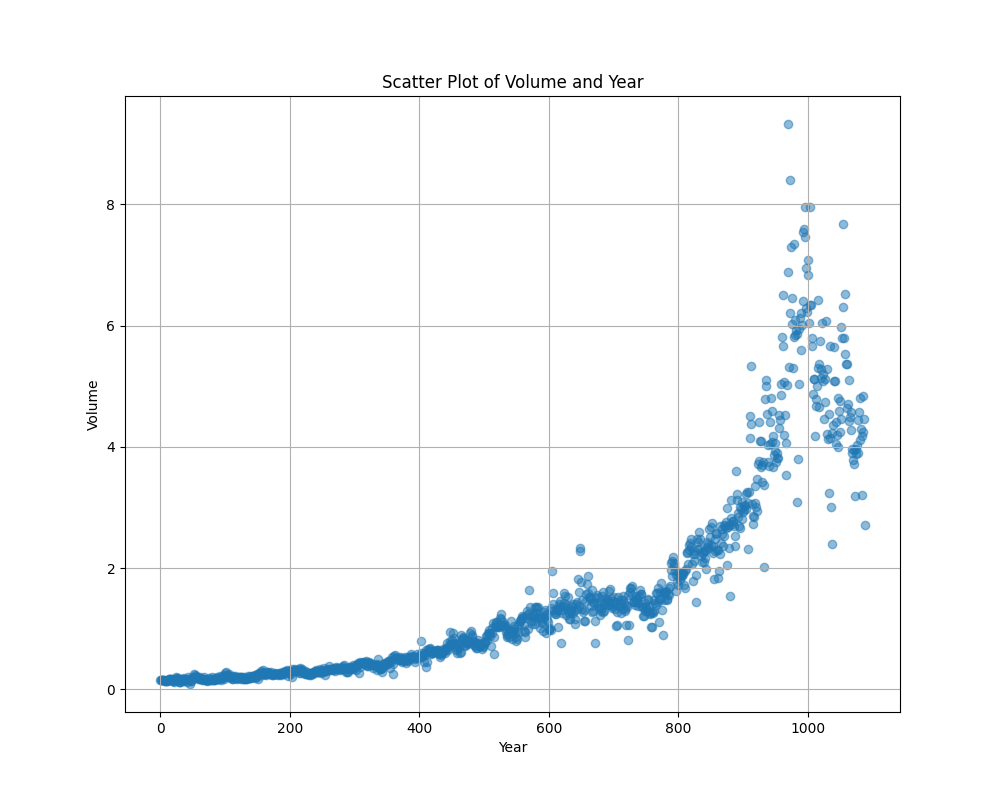
\includegraphics[width=12 cm]{graphical_correlation_analysis.png}
	\caption{Graphical Summary of Correlation between Variables}
	\label{fig_2}
\end{figure}

From Figure~\ref{fig_2}, there is relation between the variables in question. From visualization, it is clear that there is high correlation between Volume and Year. This appears to be an exponential relationship where volume increases exponentially as a function of year.\\\\
Further verification was done with Pingouin correlation package as seen in Table~\ref{table_4} and it was seen that the $R^{2}$ and and Adjusted $R^{2}$ were quite large hence indicating a high correlation between Volume and Year.

\begin{table}[h!]
 \resizebox{\textwidth}{!}{ 
\begin{tabular}{lrrlrrrlr}
	\hline
	{} &     n &         r &         CI95\% &        r2 &   adj\_r2 &          p-val &        BF10 &  power \\
	\hline
	pearson &  1089 &  0.841942 &  [0.82, 0.86] &  0.708866 &  0.70833 &  1.559688e-293 &  2.042e+289 &    1.0 \\
	\hline
\end{tabular}
}
\caption{Pearson Correlation between Volume and Year}
\label{table_4}
\end{table}

\subsection{Full Data Model}
\subsubsection{Logistic Regression (Full Model)}
Here, we will fit a logistic regression model in order to predict Direction using Lag1 through Lag5 and Volume.

\begin{table}[h!]
\centering
\begin{tabular}{llrrrrrr}
\hline
{} &      names &    coef &      se &       z &    pval &  CI[2.5\%] &  CI[97.5\%] \\
\hline
0 &  Intercept &  0.2669 &  0.0859 &  3.1056 &  0.0019 &    0.0984 &     0.4353 \\
1 &       Lag1 & -0.0413 &  0.0264 & -1.5626 &  0.1181 &   -0.0930 &     0.0105 \\
2 &       Lag2 &  0.0584 &  0.0269 &  2.1754 &  0.0296 &    0.0058 &     0.1111 \\
3 &       Lag3 & -0.0161 &  0.0267 & -0.6024 &  0.5469 &   -0.0683 &     0.0362 \\
4 &       Lag4 & -0.0278 &  0.0265 & -1.0501 &  0.2937 &   -0.0797 &     0.0241 \\
5 &       Lag5 & -0.0145 &  0.0264 & -0.5485 &  0.5833 &   -0.0662 &     0.0372 \\
6 &     Volume & -0.0227 &  0.0369 & -0.6163 &  0.5377 &   -0.0951 &     0.0496 \\
\hline
\end{tabular}
\caption{Logistic Regression (Full Model) derived using Pingouin Package}
\label{table_5}
\end{table}

So then from the variables and summary statistics in the logistic regression model output generated in Table~\ref{table_5}, we can see variables \textbf{Intercept} and \textbf{Lag2} are statistically significant which means their beta coefficients are not equal to zero. 

\subsubsection{Confusion Matrix and Prediction Analysis}
The Statsmodels and PyCM packages were used to make a prediction as to whether the market will go up or down on a particular day, we must convert these predicted probabilities
into class labels, \textbf{Up} or \textbf{Down} and create a vector of class predictions based on whether the predicted probability of a market increase.\\\\
Given these predictions, a confusion matrix was produced in order to determine how many observations were correctly or incorrectly classified. The diagonal elements of the confusion matrix indicate correct predictions, while the off-diagonals represent incorrect predictions.

\newpage

\begin{figure}[!htbp]
	\centering
	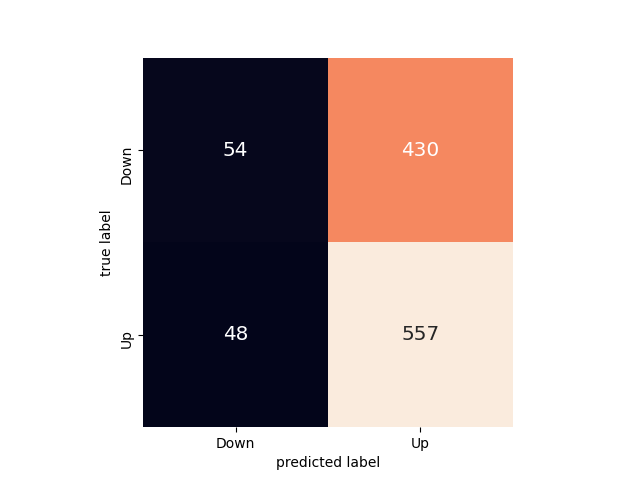
\includegraphics[width=9cm]{fullmodel.png}
	\caption{Full Model Confusion Matrix derived by Statsmodels Package}
\label{fig_3}
\end{figure} 


In using the PyCM package, it appears as though \textbf{56.1\%} of the responses are predicted correctly (model accuracy). In other words, \textbf{43.9\%} is the training error rate, which is often overly optimistic. The precision is \textbf{56.4\%} which tells that we are able to perform better than baseline.\\\\
The confusion matrix is telling us that the model does fit the data quite well. The \textbf{"Up"} direction is guessed most of the time. Most of the mistakes come from guessing that the market is going to go up when it really is going to go down. When Up is guessed, it is right \textbf{92.1\%} of the time, when down is guessed it is right \textbf{11.2\%} of the time.



\subsection{Reduced Data Model}
\subsubsection{Logistic Regression (One Predictor)}
Here, we fit the logistic regression model with Lag2 as the only predictor. 

\begin{table}[h!]
\centering
\begin{tabular}{llrrrrrr}
\hline
 &      names &    coef &      se &       z &    pval &  CI[2.5\%] &  CI[97.5\%] \\
\hline
0 &  Intercept &  0.2147 &  0.0612 &  3.5072 &  0.0005 &    0.0947 &     0.3347 \\
1 &       Lag2 &  0.0628 &  0.0264 &  2.3818 &  0.0172 &    0.0111 &     0.1145 \\
\hline
\end{tabular}
\caption{Logistic Regression (Reduced Model) dervied by Pingouin Package}
\label{table_6}
\end{table}

So then from the variables and summary statistics in the logistic regression model (reduced predictor) output generated in Table~\ref{table_6}, we can see that variables \textbf{Intercept} and \textbf{Lag2} are still statistically significant because their p values are less than 0.05. This also means their beta coefficients are not equal to zero.


\subsubsection{Confusion Matrix and Prediction Analysis}

\begin{figure}[!htbp]
	\centering
	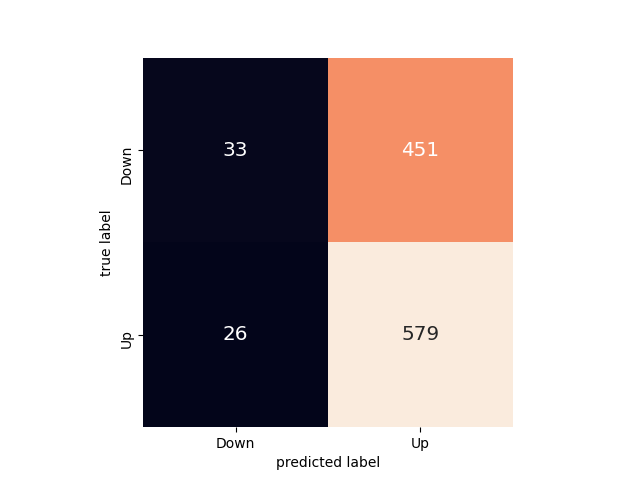
\includegraphics[width=9cm]{onemodel.png}
	\caption{Reduced Model Confusion Matrix derived by Statsmodels Package}
\label{fig_4}
\end{figure}

In using the PyCM package, it can be seen that $\textbf{56.2\%}$ of the responses are predicted correctly (model accuracy). In other words, $\textbf{43.8\%}$ is the training error rate. The precision is \textbf{56.2\%} which tells that we are able to perform better than baseline.\\\\
The confusion matrix is telling us that the model does fit the data particularly well. The \textbf{"Up"} direction is guessed most of the time. Most of the mistakes come from guessing that the market is going to go up when it really is going to go down. When Up is guessed, it is right \textbf{95.7\%} of the time, when down is guessed it is right \textbf{7.8\%} of the time.


\subsection{Interaction Data Model}
\subsubsection{Logistic Regression (Interaction Predictor)} 

Here, we fit the logistic regression model with an interaction between Lag1 and Lag2 as the only predictor. 

\begin{table}[h!]
	\centering
	\begin{tabular}{llrrrrrr}
		\hline
	{} &      names &    coef &      se &       z &    pval &  CI[2.5\%] &  CI[97.5\%] \\
	\hline
	0 &  Intercept &  0.2257 &  0.0611 &  3.6954 &  0.0002 &    0.1060 &     0.3454 \\
	1 &      Lag1*Lag2 &  0.0060 &  0.0063 &  0.9519 &  0.3411 &   -0.0063 &     0.0183 \\
		\hline
	\end{tabular}
	\caption{Logistic Regression (Interaction Predictor) dervied by Pingouin Package}
	\label{table_8}
\end{table}

So then from the variables and summary statistics in the logistic Regression (interaction predictor) output generated in the table above, we can see that no variable is statistically significant because their p values are greater than 0.05. This also means their beta coefficients are equal to zero.


\subsubsection{Confusion Matrix and Prediction Analysis}

\begin{figure}[!htbp]
	\centering
	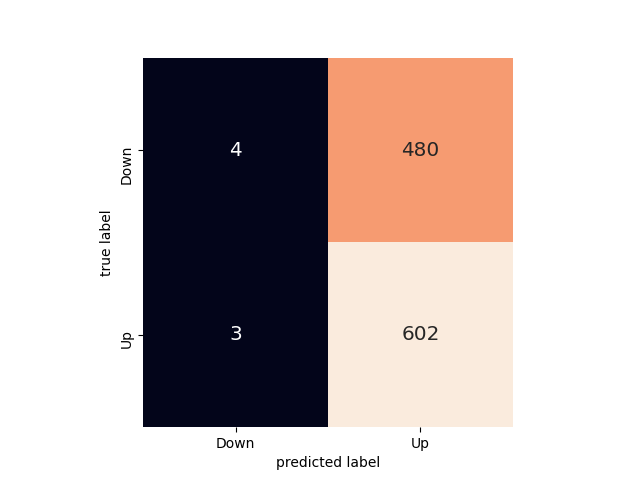
\includegraphics[width=9cm]{intmodel.png}
	\caption{Interaction Model Confusion Matrix derived by Statsmodels Package}
	\label{fig_5}
\end{figure}

From PyCM package, $\textbf{55.7\%}$ of the responses are predicted correctly (model accuracy). In other words, $\textbf{44.3\%}$ is the training error rate. The precision is \textbf{56.2\%} which tells that we are able to perform better than baseline.\\\\
The confusion matrix is telling us that the model does fit the data quite well. The \textbf{"Up"} direction is guessed most of the time. Most of the mistakes come from guessing that the market is going to go up when it really is going to go down. When Up is guessed, it is right \textbf{99.5\%} of the time, when down is guessed it is right \textbf{0.8\%} of the time.

\subsection{Performances of Methods with (Different Combinations of Predictors)}

\begin{table}[h!]
	\centering
	 \resizebox{\textwidth}{!}{ 
	\begin{tabular}{|c|c|c|c|c|c|c|}
		\hline
		Method Performance & Logistic (Full) & Logistic (One Predictor)& Logistic (Interaction) \\ 
		\hline
		Overall Fraction of Correct Prediction & 56.1\% & 56.2\%&55.7\% \\ 
		\hline
	\end{tabular} 
}
\caption{Performances of Methods with (Different Combinations of Predictors)}
\end{table}
If we compare the model accuracy (overall fraction of correct prediction), we see that \textbf{Logistic regression (One Predictor)} has the maximum model accuracy (overall fraction of correct prediction), followed by Logistic regression (Full) and Logistic (Interaction). Hence, Logistic regression (One Predictor) gives the best results.



\section{Conclusion} 
\begin{enumerate}
	\item  The research was based on the stock index over 1089 weeks for 21 years, from the beginning of 1990 to the end of 2010.  For each data,  we have recorded the percentage returns for each of the  first previous trading weeks, Lag1 through Lag5.  We have also recorded Volume (the number of shares traded on the previous day, in billions), Today (the percentage return on the date in question) and Direction (whether the market was Up or Down on this date).
	
	\item It was seen that there is no obvious pattern aside that of Volume of shares and years. 
	
	\item  It is clear that there is high correlation between Volume and Year. This appears to be an exponential relationship where volume increases exponentially as a function of year.
	
	\item It was observed that \textbf{Logistic regression (One Predictor)} has the maximum model accuracy (overall fraction of correct prediction), followed by Logistic regression (Full) and Logistic (Interaction). Hence, Logistic regression (One Predictor) gives the best results.
\end{enumerate}







\begin{thebibliography}{999}

	% Reference 1
	\bibitem[Wikipedia contributors (2020)]{ref-wiki}
	Wikipedia contributors.(2020). S\&P 500 Index. In Wikipedia, The Free Encyclopedia. Online; accessed 28-July-2020, from {\url{https://en.wikipedia.org/w/index.php?title=S\%26P_500_Index&oldid=969280492}}
	
	% Reference 2
	\bibitem[Duggan, Wayne (2019)]{ref-quote}
	Duggan, Wayne (2019). (June 13, 2019). "This Day In Market History: S\&P 500 Quotes Delivered Every 15 Seconds", on June 13, 2019. Benzinga.
	
	% Reference 3
	\bibitem[Wikipedia contributors (2020)]{ref-wiki:xxx}
	Wikipedia contributors.(2020). Logistic regression. In Wikipedia, The Free Encyclopedia Online; accessed 28-July-2020, from  {\url{https://en.wikipedia.org/w/index.php?title=Logistic\_regression\&oldid=967311267}}
	
	% Reference 4
	\bibitem[Vallat, R. (2018)]{ref-software}
	Vallat, R. (2018). Pingouin: statistics in Python. Journal of Open Source Software, 3(31), 1026, {\url{https://doi.org/10.21105/joss.01026}}
	
	% Reference 5
	\bibitem[Haghighi et al., (2018)]{ref-softwaree}
	Haghighi et al., (2018). PyCM: Multiclass confusion matrix library in Python. Journal of Open Source Software, 3(25), 729.
	{\url{https://doi.org/10.21105/joss.00729}}
\end{thebibliography}
\end{document}

